\documentclass[10pt,a4paper]{article}
\usepackage[T1]{fontenc}
\usepackage[utf8]{inputenc}
\usepackage{graphicx}
\usepackage{tabularx}
\usepackage{helvet}
\usepackage{hyperref}
\usepackage[a4paper,margin=1in]{geometry}
\usepackage[polish]{babel}
\usepackage{float}
\usepackage{xcolor}
\usepackage{listings}
\usepackage{inconsolata}
\lstdefinestyle{bash}{
  basicstyle=\ttfamily\color{black},
  captionpos=b,
  commentstyle=\color{teal},
  keywordstyle=\color{blue},
  stringstyle=\color{olive},
  language=bash,
  moredelim=**[is][\color{blue}]{^}{^},
  showstringspaces=false,
  columns=fullflexible
}

\renewcommand\familydefault{\sfdefault}

\title{Linux w systemach wbudowanych -- Laboratorium 4}
\author{Tymon Felski}

\begin{document}

\makeatletter
\begin{center}
	\LARGE{\@title}\\
	\vspace{.4cm}
	\Large{\@author}\\
	\vspace{.2cm}
	\large{\today}
\end{center}
\makeatother

\section{Treść zadania}
Podczas czwartego laboratorium należało przygotować przy pomocy płytki Raspberry Pi urządzenie wyposażone w złożony interfejs użytkownika, w którym:
\begin{itemize}
	\item przyciski i diody LED powinny być użyte do podstawowej obsługi urządzenia,
	\item interfejs WWW lub inny interfejs sieciowy powinien być użyty do bardziej zaawansowanych funkcji,
	\item przetwarzany powinien być dźwięk lub obraz.
\end{itemize}

\section{Odtwarzanie projektu z załączonego archiwum}
Dostarczone archiwum należy umieścić w dowolnym miejscu na dysku i rozpakować. Uruchomienie skryptu \texttt{install.sh}, znajdującego się w środku archiwum, spowoduje odtworzenie konfiguracji środowiska z laboratorium. Jako parametr należy podać ścieżkę do katalogu z rozpakowanymi plikami Buildroota.\\[\baselineskip]
Skrypt utworzy katalog \texttt{felskit-lab4/} równoległy do katalogu przekazanego jako argument. Następnie do obu z nich zostaną przekopiowane odpowiednie pliki i katalogi. Ponadto, skrypt zastosuje domyślną konfigurację dla płytki Raspberry Pi i właściwie spatchuje pliki konfiguracyjne Buildroota. Na koniec skrypt zapyta czy rozpocząć kompilację jądra systemu.

\section{Opis rozwiązania}
\subsection{Przygotowanie}
W celu przygotowania środowiska Buildroot, ustawiono następujące opcje:
\begin{enumerate}
	\item \textit{System configuration} $\rightarrow$ \textit{Port to run a getty (login prompt) on} na \textit{ttyAMA0}
	\item \textit{Build options} $\rightarrow$ \textit{Mirrors and Download locations} $\rightarrow$ \textit{Primary download site}\\
	na \textit{http://192.168.137.24/dl}
	\item \textit{Target options} $\rightarrow$ \textit{Target ABI} na \textit{EABI}
	\item \textit{Toolchain} $\rightarrow$ \textit{Toolchain type} na \textit{External toolchain}
	\item \textit{Toolchain} $\rightarrow$ \textit{Toolchain} na \textit{Sourcery CodeBench ARM 2014.05}
\end{enumerate}
Ponadto, zaznaczono opcję
\begin{quote}
	\textit{Filesystem images} $\rightarrow$ \textit{initial RAM filesystem linked into linux kernel}
\end{quote}
oraz włączono kompresję obrazu ustawiając opcję
\begin{quote}
	\textit{Filesystem images} $\rightarrow$ \textit{tar the root filesystem, Compression method (gzip)}
\end{quote}

\subsection{Zadania}
\subsubsection{Aplikacja}
Stworzona w ramach laboratorium aplikacja to internetowe radio napisane w Pythonie, którym można sterować przy pomocy interfejsu \texttt{GPIO} oraz interfejsu webowego. Do obsługi przycisków i diod LED na płytce Raspberry Pi wykorzystano pythonowy moduł \texttt{RPi.GPIO}, natomiast interfejsem webowym zarządza framework \texttt{Flask}.\\[\baselineskip]
Przycisk o numerze pinu 27 służy do zmiany stacji na następną, a przyciski o numerach 10 i 22 odpowiednio zmniejszają i zwiększają głośność odtwarzania. Interfejs webowy jest bardziej rozbudowany i udostępnia dodatkowe funkcjonalności, takie jak zmiana stacji na poprzednią, wybranie konkretnej stacji z listy oraz całkowite zatrzymanie streamu.\\[\baselineskip]
Oba interfejsy wyświetlają aktualnie graną stację radiową i głośność odtwarzania. Diody LED na płytce Raspberry Pi odzwierciedlają obecną głośność odtwarzania, gdzie przy głośności 0\% wszystkie diody będą zgaszone, a przy 100\% - zapalone.\\[\baselineskip]
Interfejs webowy, zdefiniowany w pliku \texttt{templates/main.html}, wykorzystuje \texttt{jQuery} i style \texttt{Bootstrapowe}, dzięki czemu jest responsywny. Dodatkowa część zadania wymagała dodania \texttt{HTML-owego} formularza, przyjmującego dwa napisy, do interfejsu webowego oraz obsługi odpowiedniego zapytania typu \texttt{POST} po stronie serwera. Po wpisaniu nazwy stacji i adresu pod którym można znaleźć stream oraz wciśnięciu przycisku \texttt{Submit}, stacja zostanie dodana do listy widocznej pod głównym panelem.
\begin{figure}[H]
	\centering
	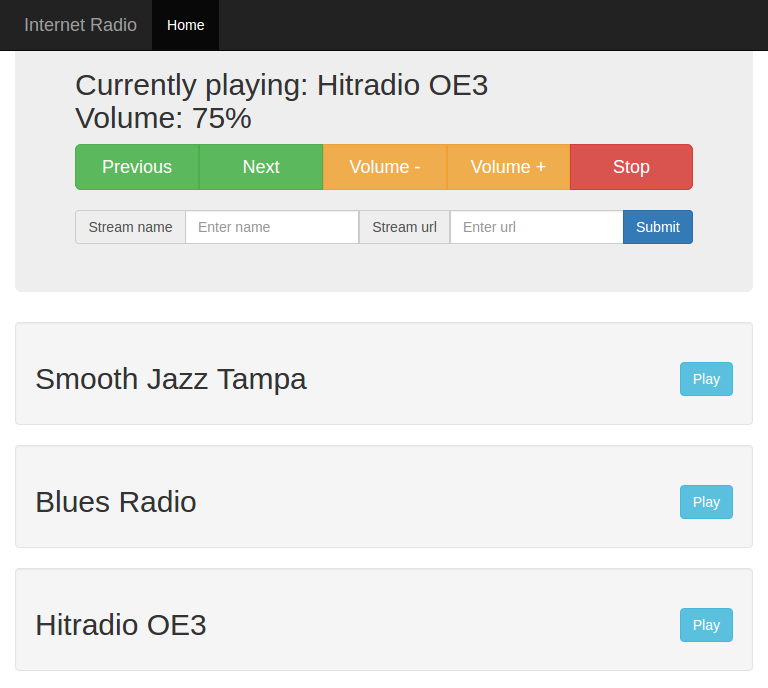
\includegraphics[width=10cm]{web-ui.png}
	\caption{Zrzut ekranu interfejsu webowego}
\end{figure}
\noindent
Stacje radiowe są wczytywane z pliku \texttt{stations.txt} na początku działania aplikacji. Muzyka jest odtwarzana przy pomocy \texttt{mpc}, prostego klienta do \texttt{mpd} (\textit{Music Player Deamon}), który z kolei jest skonfigurany do współpracy z \texttt{ALSA} (\textit{Advanced Linux Sound Architecture}). Pythonowe funkcje obsługujące odtwarzacz korzystają z pomocniczej funkcji \texttt{run\_cmd}, która przy pomocy modułu \texttt{subprocess} tworzy proces potomny do wykonywania komend w linii poleceń.
\begin{lstlisting}[style=bash, language=python, caption={Funkcja pomocnicza run\_cmd}]
def run_cmd(cmd):
    p = Popen(cmd, shell=True, stdout=PIPE, stderr=STDOUT)
    output = p.communicate()[0]
    return output
\end{lstlisting}
Przygotowano trzy wersje aplikacji. Pierwsza, której źródło znajduje się w pliku \texttt{radio-blocking.py}, działa na czterech wątkach, z których trzy obsługują przyciski na płytce Raspberry Pi przy pomocy blokujących funkcji \texttt{wait\_for\_edge}, a na czwartym działa serwer \texttt{Flaskowy}. Niestety ze względu na występujący obecnie \href{https://sourceforge.net/p/raspberry-gpio-python/tickets/103/}{problem} w module obsługującym interfejs \texttt{GPIO}, nie jest możliwe, aby wszystkie trzy wątki czekały jednocześnie na wciśnięcie przycisku.
\begin{lstlisting}[style=bash, caption={Funkcje obsługujące interfejs GPIO (z radio-blocking.py)}]
^def^ gpio10_handler():
    while True:
        GPIO.wait_for_edge(10, GPIO.FALLING)
        ^with^ lock:
            mpc_vol_down()
            mpc_print()

^def^ gpio22_handler():
    while True:
        GPIO.wait_for_edge(22, GPIO.FALLING)
        ^with^ lock:
            mpc_vol_up()
            mpc_print()

^def^ gpio27_handler():
    while True:
        GPIO.wait_for_edge(27, GPIO.FALLING)
        ^with^ lock:
            mpc_next()
            mpc_print()
\end{lstlisting}
Druga wersja aplikacji, która znajduje się w pliku \texttt{radio-polling.py} jest modyfikacją poprzedniej. Interfejs \texttt{GPIO} jest obsługiwany przez jeden wątek, który odpytuje przyciski pięć razy na sekundę. Pozostała część aplikacji została zrealizowana w ten sam sposób.
\begin{lstlisting}[style=bash, caption={Funkcje obsługujące interfejs GPIO (z radio-polling.py)}]
^def^ poll_btns():
    if GPIO.input(10) == GPIO.LOW:
        return "down"
    if GPIO.input(22) == GPIO.LOW:
        return "up"
    if GPIO.input(27) == GPIO.LOW:
        return "next"
    return "none"

^def^ gpio_handler():
    global exit
    while not exit:
        pressed = poll_btns()
        if pressed != "none":
            ^with^ lock:
                if pressed == "down":
                    mpc_vol_down()
                elif pressed == "up":
                    mpc_vol_up()
                else:
                    mpc_next()
                mpc_print()
        time.sleep(0.2)
\end{lstlisting}
\newpage
\noindent
Trzecia wersja, znajdująca się w pliku \texttt{radio-events.py}, korzysta z jednego wątku do obsługi serwera, jednak przed jego uruchomieniem zapisuje przy pomocy \texttt{add\_event\_detect} trzy funkcje obsługujące interfejs \texttt{GPIO} na eventy odpowiadające wciśnięciu odpowiednich przycisków. W ten sposób w aplikacji nie ma oczekiwania aktywnego, a callbacki wywołają się na dodatkowych wątkach w przypadku wciśnięcia któregoś z przycisków.
\begin{lstlisting}[style=bash, caption={Funkcje (callbacki) obsługujące interfejs GPIO (z radio-events.py)}]
^def^ gpio10_handler():
    ^with^ lock:
        mpc_vol_down()
        mpc_print()

^def^ gpio22_handler():
    ^with^ lock:
        mpc_vol_up()
        mpc_print()

^def^ gpio27_handler():
    ^with^ lock:
        mpc_next()
        mpc_print()
\end{lstlisting}
Wszystkie wersje zostały wyposażone w handler przerwania. Funkcja \texttt{register} z modułu \texttt{atexit} zapisuje przekazają jako argument funkcję \texttt{interrupt} na event odpowiadający wciśnięciu \texttt{\^}\texttt{C}. Odpowiada ona za wyczyszczenie zasobów, czyli przywrócenie początkowych stanów pinów \texttt{GPIO} oraz zatrzymanie odtwarzania muzyki. Wątki w wersjach 1. i 2. są uruchamiane z parametrem \texttt{daemon = True}, który powoduje, że główny wątek nie musi czekać na ich zakończenie (zostają one zabite razem z nim). Mimo to w wersji 2. zastosowano zakończenie wątku przy pomocy flagi logicznej i wywołanie funkcji \texttt{join}. W wersji 3. funkcja \texttt{interrupt} dodatkowo wyrejestrowuje callbacki obsługujące interfejs \texttt{GPIO}.
\begin{lstlisting}[style=bash, language=python, caption={Przykładowy handler przerwania (z radio-events.py)}]
def interrupt():
    for button in [10, 22, 27]:
        GPIO.remove_event_detect(button)
    GPIO.cleanup()
    mpc_stop()
\end{lstlisting}
Serwer \texttt{Flaskowy} działa na zasadzie komunikacji poprzez zapytania. Do danych ścieżek przypisane są pythonowe funkcje. Zostają one wywołane, przetwarzają zapytanie i odpowiadają na nie, co skutkuje wyświetleniem odpowiedniej strony w przeglądarce po stronie użytkownika. Wszystkie funkcje są zabezpieczone przy pomocy mechanizmu \texttt{Reentrant Lock}, aby aplikacja mogła działać równolegle z wątkami obsługującymi interfejs \texttt{GPIO}.

\subsubsection{Obraz systemu}
Obraz systemu musiał zostać wyposażony w szereg narzędzi i paczek, aby mógł odtwarzać dźwięk i uruchomić wcześniej opisywaną aplikację. Dodanie interpretera języka skryptowego Python do obrazu systemu polega na zaznaczeniu opcji
\begin{quote}
\textit{Target packages} $\rightarrow$ \textit{Interpreter languages and scripting} $\rightarrow$ \textit{python3}
\end{quote}
Następnie zaznaczono opcje odpowiadające niezbędnym pythonowym modułom
\begin{quote}
\textit{Target packages} $\rightarrow$ \textit{Interpreter languages and scripting} $\rightarrow$ \textit{External python modules} $\rightarrow$ \textit{python-rpi-gpio}\\
\textit{Target packages} $\rightarrow$ \textit{Interpreter languages and scripting} $\rightarrow$ \textit{External python modules} $\rightarrow$ \textit{python-flask}
\end{quote}
Odtwarzacz muzyki \texttt{mpd} wraz z wymaganym klientem \texttt{mpc} można znaleźć pod opcjami
\begin{quote}
\textit{Target packages} $\rightarrow$ \textit{Audio and video applications} $\rightarrow$ \textit{mpd}\\
\textit{Target packages} $\rightarrow$ \textit{Audio and video applications} $\rightarrow$ \textit{mpd-mpc}
\end{quote}
Aby \texttt{mpc} mógł obsługiwać streamy stacji radiowych z internetu wymagany jest plugin \texttt{curl}, który można wybrać zaznaczając
\begin{quote}
\textit{Target packages} $\rightarrow$ \textit{Audio and video applications} $\rightarrow$ \textit{mpd (Input plugins)} $\rightarrow$ \textit{curl}
\end{quote}
Współdziałanie \texttt{mpd} oraz \texttt{ALSA} zapewni opcja
\begin{quote}
\textit{Target packages} $\rightarrow$ \textit{Audio and video applications} $\rightarrow$ \textit{mpd (Output plugins)} $\rightarrow$ \textit{alsa}
\end{quote}
Wybranie powyższej opcji powinno automatycznie zaznaczyć
\begin{quote}
\textit{Target packages} $\rightarrow$ \textit{Libraries} $\rightarrow$ \textit{Audio/Sound} $\rightarrow$ \textit{alsa-lib}
\end{quote}
Konieczne jest także dodanie
\begin{quote}
\textit{Target packages} $\rightarrow$ \textit{Audio and video applications} $\rightarrow$ \textit{alsa-utils}
\end{quote}
Wybrano ponadto pomocnicze paczki potomne \texttt{alsa-utils}, takie jak \textit{alsaconf}, \textit{alsactl}, \textit{alsamixer}, \textit{amixer} oraz \textit{aplay}.\\[\baselineskip]
Aplikację umieszono w obrazie systemu przy pomocy mechanizmu Overlay. W opcji
\begin{quote}
\textit{System configuration} $\rightarrow$ \textit{Root filesystem overlay directories}
\end{quote}
podano ścieżkę do katalogu \texttt{overlay/}, do którego zostały skopiowane wszystkie pliki źródłowe.\\[\baselineskip]
Konfiguracja \texttt{mpd} wymagała zdefiniowania urządzenia wyjściowego korzystającego z \texttt{ALSA}. Dodano plik \texttt{/etc/mpd.conf} rozszerzony o linie
\begin{lstlisting}[style=bash, keywordstyle=\color{black}]
audio_output {                                                                  
        type            "alsa"
        name            "ALSA Device"
        mixer_type      "software"
}
\end{lstlisting}
Został on utworzony na podstawie domyślnego pliku \texttt{mpd.conf} wygenerowanego podczas kompilacji obrazu systemu. Przed końcem kompilacji domyślna wersja tego pliku zostanie nadpisana tą z katalogu \texttt{overlay/}.\\[\baselineskip]
Ostatnim krokiem było zmodyfikowanie \texttt{device tree} generowanego podczas kompilacji. Przy pomocy \texttt{dtc} (\textit{Device Tree Compiler}) rozkompilowano plik \texttt{bcm2708-rpi-b.dtb} poleceniem
\begin{lstlisting}[style=bash, commentstyle=\color{black}]
# dtc -I dtb -O dts -o bcm2708-rpi-b.dts bcm2708-rpi-b.dtb
\end{lstlisting}
Następnie znaleziono opcję \texttt{status} odpowiadającą \texttt{brcm,bcm2835-audio} i zmieniono jej wartość z \texttt{disabled} na \texttt{okay}, po czym ponownie skompilowano plik poleceniem
\begin{lstlisting}[style=bash, commentstyle=\color{black}]
# dtc -I dts -O dtb -o bcm2708-rpi-b.dtb bcm2708-rpi-b.dts
\end{lstlisting}
Tak zmodyfikowany plik \texttt{bcm2708-rpi-b.dtb} mógł zostać umieszczony na karcie pamięci płytki Raspberry Pi obok obrazu \texttt{zImage}.

\subsubsection{Konfiguracja}
Po uruchomieniu obrazu systemu należy załadować moduł jądra odpowiedzialny za dźwięk przy pomocy polecenia
\begin{lstlisting}[style=bash, commentstyle=\color{black}]
# modprobe snd_bcm2835
\end{lstlisting}
Wówczas jeżeli widoczna jest karta dźwiękowa, a \texttt{mpd} oraz \texttt{alsa} działają poprawnie, można uruchomić radio jednym z plików o rozszerzeniu \texttt{.py} po przełączeniu się do katalogu \texttt{/radio}.

\end{document}
